\section{Introduction}

  Ordinary differential equations model deterministic systems that can be solved exactly through integration. For example, consider the population model determined by a linear DEQ 

    \begin{equation}
      \frac{d N} {dt} = \alpha(t) N (t)
    \end{equation}

  where $N$ is the population size and $\alpha$ is a growth rate. Then, we can solve with analysis by integrating the following with a change of basis

  \begin{align*}
    \int \frac{1}{N(t)} \frac{dN}{dt} \,dt = \int \alpha(t) \,dt \iff \int \frac{1}{N} \, dN = \int \alpha(t) \,dt \\
    & \iff N(t) = C \exp \bigg( \int \alpha (t) \,dt \bigg) 
  \end{align*}
  
  This classical exponential growth model is not only continuous, but \textit{smooth}, and it is this smoothness that allows us to do calculus on it. But more realistic models will have noise, which can be modeled by a \hyperref[prob-def:random-variable]{random variable}. Let $\alpha = r + \eta$, where $r$ is the deterministic term and $\eta$ is the random term. Then, integrating gives us 

    \begin{equation}
      \frac{dN}{dt} = \big( r(t) + \eta(t) \big) N(t) \iff \int \frac{1}{N} \frac{dN}{dt} \,dt = \int r(t) \,dt + \int \eta(t) \,dt
    \end{equation}
    
  The first integral can be evaluated, but classical calculus does not allow us to integrate the random part. This is where stochastic calculus is needed. Now recall from probability that a random variable over a \hyperref[prob-def:probability-space]{probability space} $(\Omega, \mathcal{F}, \mathbb{P})$ is simply a $\mathcal{F}$-measurable function $X$. As some warm up exercises, let us prove a few examples. 

  \begin{example}[Class 1]
    \label{ex:class-1}
 
    
  \end{example}

  \begin{example}[Class 2]
    \label{ex:class-2}
    
  \end{example}

  \begin{definition}[Stochastic Process]
    \label{def:stochastic-process}
    A \textbf{stochastic process} is a collection of \hyperref[prob-def:random-variable]{random variables} indexed by time $\{X_t\}_{t \in T}$ with their respective measures $\rho_t$. 

    \begin{enumerate}
      \item If $T$ is countable (usually integers), then it is called a \textbf{discrete-time} stochastic process. 
      \item If $T$ is continuous, then it is called a \textbf{continuous-time} stochastic process. 
    \end{enumerate}

    It is also good to think of it as a probability distribution over a space of paths. 
  \end{definition}

  \begin{definition}[Filtration]
    \label{def:filtration}
    Let $(\Omega, \mathcal{F}, \mathbb{P})$ be a \hyperref[prob-def:probability-space]{probability space} and $I$ be an index set with \hyperref[st-def:total-order]{total order} $\geq$ (usually, $\mathbb{N}, \mathbb{R}$). For every $i \in I$, let $\mathcal{F}_i$ be a sub-$\sigma$-algebra of $\mathcal{F}$ satisfying 
    \begin{equation}
      \mathcal{F}_i \subset \mathcal{F}_j \text{ if } i \geq j
    \end{equation}
    Note that we do not write it as a sequence like before since $I$ may be uncountable. Then, a \textbf{filtration} $\mathbb{F} = \{\mathcal{F}_i\}_{i \in I}$ is a family of $\sigma$-algebras that are ordered nondecreasingly. If $\mathbb{F}$ is a filtration, then $(\Omega, \mathcal{F}, \mathbb{F}, \mathbb{P})$ is called a \textbf{filtered probability space}. A \hyperref[def:stochastic-process]{stochastic process} $(X_t)_{t \in I}$ is \textbf{adapted} to $\mathbb{F}$ if for every $t \in I$, $X_t$ is $\mathcal{F}_t$-measurable. 
  \end{definition}

  We first start off with Markov processes. We can divide them into four kinds, depending on whether we are using discrete or continuous time, and whether we are using discrete or continuous state space. Since process over continuous state space is a natural generalization of those in a discrete one, we only distinguish between the times. When talking about continuous time, there are additional operators we must introduce, such as generators. Before we go any further, I would like to mention that these notes write the transition matrices of \hyperref[def:markov-chain]{Markov chains} as \textbf{row-stochastic} (right-stochastic) matrices, which is the usual convention. Therefore, a \hyperref[def:transition-matrix]{transition matrix} looks like 

    \begin{equation}
      \mathbf{P} = \begin{pmatrix} P(1, 1) & \ldots & P(1, d) \\ \vdots & \ddots & \vdots \\ P(d, 1) & \ldots & P(d, d) \end{pmatrix}
    \end{equation}

  where $P(i, j)$ represents the probability of transition from state $i$ to state $j$, so that each row sums to $1$. Distributions are then row vectors acting on the right, $\boldsymbol{\rho}^T \mathbf{P}$, and functions are column vectors acting on the left, $\mathbf{P} \mathbf{f}$. I use this notation because it is consistent with when we are working with Markov processes over general measurable state spaces. Note that we will denote in math font general objects and operators ($X_t, \rho_t, P_s, \pi$) and their realization as vectors and matrices in bold font ($\boldsymbol{\rho_t}, \mathbf{P_s}, \boldsymbol{\pi}$). 

  \subsection{Transitioning from Discrete to Continuous State Space}

    Let us remind ourselves of the definitions involving Markov chains over a discrete state space. Let $X_t$ be the state at time $t$. The discrete distribution of $X_t$ can be represented as a \hyperref[lin-def:column-vector]{column vector} $\boldsymbol{\rho_t}$, where $\boldsymbol{\rho_t} (i) = \mathbb{P}(X_t = i)$, and we can calculate the distribution of $X_{t + s}$ as 

      \begin{equation}
        \boldsymbol{\rho_{t + s}}^T = \boldsymbol{\rho_{t}}^T \boldsymbol{P_s}
      \end{equation}

    where $\boldsymbol{P_s}$ is a stochastic matrix. Note that representing a discrete measure on discrete $S = \{1, \ldots, d\}$ with a vector really just a notational convenience for computations. We must properly distinguish the three: 

    \begin{enumerate}
      \item the actual state $X_t$ 
      \item the probability distribution $\rho_t$, which is a measure 
      \item the PMF vector $\boldsymbol{\rho_t}$, which is just a convenient representation of $\rho_t$ in the way that 
      \begin{equation}
        \boldsymbol{\rho_t} (i) = \rho_t (\{i\}) = \mathbb{P}(X_t = i)
      \end{equation}
      That is, the $i$th element is just the measure on the singleton set $\{i\} \in \mathcal{S} = 2^S$. 
    \end{enumerate}

    The PMF vector $\boldsymbol{\rho_t}$ is really just a way to describe $X_t$ and its distribution, which is redundant. Furthermore, when we try to describe states $X_t$ in general \hyperref[mt-def:measure-space]{measure spaces} $(S, \mathcal{S})$, we cannot think of it as a vector anymore. This is not a problem in even countable spaces since we can just assign $\boldsymbol{\rho_t} (i) = \mathbb{P}(X_t = i)$ in a finite space, but for uncountably infinite spaces we cannot do this. Therefore, we must have some measurable \textbf{function} $f: S \rightarrow \mathbb{R}$ that extracts this kind information from $X_{t}$. Therefore, we must really work with the following: 

    \begin{enumerate}
      \item the actual state $X_t: (\Omega, \mathcal{F}, \mathbb{P}) \to (S, \mathcal{S})$ 
      \item the probability distribution $\rho_t$ of the state $X_t$ 
      \item a collection of $\mathcal{S}$-measurable functions $f: S \to \mathbb{R}$ that describes the state 
    \end{enumerate}

    At this point, we are not sure what $f$ is since it seems quite arbitrary. But if we fix some $A \in \mathcal{S}$ and take $f = 1_A$, then $1_A (X_t)$ encodes the information of whether $X_t$ is in $A$ or not. This is quite nice, since now we can think of the PMF vector $\boldsymbol{\rho_t}$ as having components defined by the functions 

      \begin{equation}
        \boldsymbol{\rho_t} (i) = 1_{\{i\}} (X_t) = \mathbb{P}(X_t = i)
      \end{equation}

    The following theorem formalizes this concept. 

    \begin{theorem}[Equality of Distributions via Expectations]
      \label{thm:equality-of-distributions-via-expectations}
      Two \hyperref[prob-def:random-variable]{random variables} $X, Y : (\Omega, \mathcal{F}, \mathbb{P}) \rightarrow (S, \mathcal{S})$ have the same distribution if 

        \begin{equation}
          \mathbb{E}[f(X)] = \mathbb{E}[f(Y)]
        \end{equation}

      for all $\mathcal{F}$-measurable $f: S \rightarrow \mathbb{R}$, which can be seen by setting $f = 1_A$ for any $A \in \mathcal{F}$. 

      \begin{align*}
        \mathbb{E}[1_A (X)] = \mathbb{E}[1_A (Y)] & \implies \mathbb{P}(X \in A) = \mathbb{P}(Y \in A) \\
        & \implies \mathbb{P}_X (A) = \mathbb{P}_Y (A)
      \end{align*}
      and so the measure that $X$ and $Y$ pushes forward to $(S, \mathcal{S})$ is precisely the same. This does not mean that they are the same random variable. 
    \end{theorem}

    Let's talk more about $f$ in the discrete case setting. We know that the discrete distributions are represented by a \hyperref[lin-def:column-vector]{column vector}. It is true that every \hyperref[mt-def:measurable-function]{measurable function} can be written as a \hyperref[lin-def:linear-combination]{linear combination} of simple (indicator) functions, and so in a discrete space $S = \{1, \ldots, d\}$, we can write every $f$ as 

      \begin{equation}
        f = \sum_{i \in S} f_i 1_{\{i\}}
      \end{equation}

    which outputs $f_i$ if its input is $i$. We can interpret it as a column vector $\mathbf{f} = (f_1, \ldots, f_d)^T$ . We can see that 

      \begin{equation}
        \boldsymbol{\rho_t}^T \mathbf{f} = \begin{pmatrix} \boldsymbol{\rho_t} (1) & \ldots & \boldsymbol{\rho_t} (d) \end{pmatrix} \begin{pmatrix} f_1 \\ \vdots \\ f_d \end{pmatrix} = \mathbb{E}[f(X_t)]
      \end{equation}

    and if $\mathbf{f}$ is any standard unit vector, say $(1, 0, 0)$ with $d = 3$, then

      \begin{equation}
        \boldsymbol{\rho_t}^T \mathbf{f}  = \begin{pmatrix} \boldsymbol{\rho_t} (1) & \boldsymbol{\rho_t} (2) & \boldsymbol{\rho_t} (3) \end{pmatrix} \begin{pmatrix} 1 \\ 0 \\ 0 \end{pmatrix}= \mathbb{E}[1_{\{1\}} (X_t)] = \mathbb{P}(X_t = 1)
      \end{equation}

    Therefore, every time we compute $\mathbb{E}[f(X_t)]$, we can think of it in the discrete case as dotting $\boldsymbol{\rho_t}$ with a function vector $\mathbf{f}$ to extract whatever we want from the vector $X_t$. And as we will find out later, the linearity of the stochastic matrix $\mathbf{P_s}$ is analogous to the linearity of the Markov \hyperref[alg-def:semigroup]{semigroup} $P_s$.  

    Therefore, our Markov process is really just some \hyperref[def:stochastic-process]{stochastic process} $\{X_t\}_{t \geq 0}$ over some measurable space $(S, \mathcal{S})$ with the property that 

      \begin{equation}
        \mathbb{P}(X_{t + s} \in A \mid \{X_r \in B_r\}_{r \leq t}) = \mathbb{P}( X_{t + s} \in A \mid X_t \in B_t)
      \end{equation}

    where $A \in \mathcal{S}$, and this captures the discrete case by setting $A = \{j\} \in 2^S$ which gives 

      \begin{equation}
        \mathbb{P}( X_{t + s} = j \mid \{X_r = i_r\}_{r \leq t}) = \mathbb{P}( X_{t + s} = j \mid X_t = i_t)
      \end{equation}

    This basically says that the probability that $X_{t + s}$ lying in $A$ is only dependent on its present state $X_t \in B_t$, not the history $\{X_r \in B_r\}_{r \leq t}$. In fact, by using the identity $\mathbb{E}[1_A] = \mathbb{P}(A)$ and setting $f = 1_A$, we can capture this effect for \textit{all} measurable $f: (S, \mathcal{S}) \rightarrow (\mathbb{R}, \mathcal{R})$. Thus, the \hyperref[def:markov-property]{Markov property} now looks like  

      \begin{equation}
        \mathbb{E}[f (X_{t + s}) \mid \{X_r \in B_r\}_{r \leq t}] = \mathbb{E}[ f(X_{t + s}) \mid X_t \in B_t]
      \end{equation}

    We don't need to fix the $X_r$'s into sets $B_r$'s and so we can write 

      \begin{equation}
        \mathbb{E}[f (X_{t + s}) \mid \{X_r\}_{r \leq t}] = \mathbb{E}[ f(X_{t + s}) \mid X_t]
      \end{equation}


    Now let's talk about this Markov property. It is true that $\sigma$-algebra $\sigma(\{X_r\}_{r \leq t})$ is bigger than $\sigma(X_t)$; the Markov property does not imply that they are the same size. Rather, we should interpret this as the extra information introduced by the bigger $\sigma(\{X_r\}_{r \leq})$ is irrelevant. This is analogous to trying to approximate a function with a pointlessly large $\sigma$-algebra. For example, given a piecewise function $X$ defined on the unit interval $\Omega = [0, 1]$, let $\mathcal{G}$ be the $\sigma$-algebra generated by $[0, 0.5), [0.5, 1]$ and $\mathcal{H}$ be that generated by $[0, 0.25), [0.25, 0.5), [0.5, 0.75), [0.75, 1]$. 

    \begin{center}
      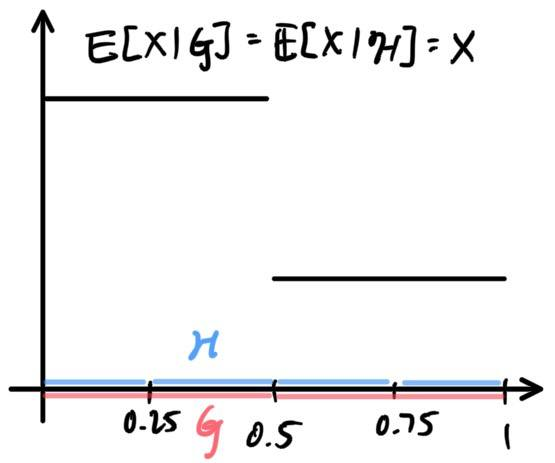
\includegraphics[scale=0.3]{img/pointless_approximation.jpg}
    \end{center}

    Then, we can see that 

      \begin{equation}
        \mathbb{E}[X \mid \mathcal{G}] = \mathbb{E}[X \mid \mathcal{H}]
      \end{equation}

    That is, the two \hyperref[prob-def:random-variable]{random variables} are exactly equal, even though $\mathcal{H}$ has more information than $\mathcal{G}$. Note that this is not the law of iterated expectations. This rule does not say that $\mathbb{E}[\mathbb{E}[X \mid \mathcal{G}]] = \mathbb{E}[ \mathbb{E}[X \mid \mathcal{H}]]$; this law is true regardless. Rather, this property is a special property of the function $X$, and therefore the Markov property is a special property of the stochastic process $\{X_t\}_{t \geq 0}$. 
